
%(BEGIN_QUESTION)
% Copyright 2006, Tony R. Kuphaldt, released under the Creative Commons Attribution License (v 1.0)
% This means you may do almost anything with this work of mine, so long as you give me proper credit

Analyser denne elektroniske sensoren for termisk ledningsevne, brukt til å detektere ulike kjemiske komponenter som kommer ut av kolonnen i en kromatograf. Både målefilamentet og referansefilamentet varmes av strømmen som går gjennom dem, og en variabel spenning utvikles over hver av dem ettersom gassene kjøler dem ulikt:

$$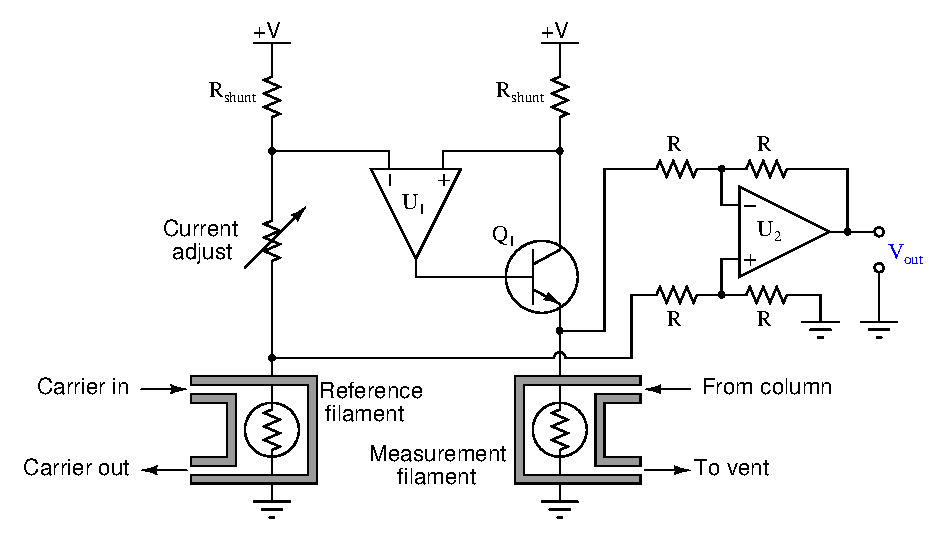
\includegraphics[width=15.5cm]{i00678x01.eps}$$

Forklar følgende om denne kretsen:

\begin{itemize}
\item{} Hvordan justerer reostaten strømmen likt gjennom {\it begge} filamentene?
\item{} Hvordan samarbeider op-amp $U_1$ og transistor $Q_1$ for å regulere strømmen gjennom målefilamentet?
\item{} Hvordan kan vi se at op-amp $U_1$ faktisk går i negativ tilbakekobling, når det ved første blikk kan se ut som positiv tilbakekobling fordi $R_{shunt}$-signalet går til ikke-inverterende (+) inngang?
\item{} Hva er funksjonen til op-amp $U_2$ og de fire like store motstandene?
\item{} Hvor i denne kretsen måles et utgangsspenningssignal?
\item{} Hvilken retning går utgangsspenningen når målefilamentet blir varmere enn referansefilamentet, gitt positiv temperaturkoeffisient for motstand ($\alpha$) i filamentmetallet?
\end{itemize}

\underbar{file i00678no}
%(END_QUESTION)





%(BEGIN_ANSWER)

\begin{itemize}
\item{} Hvordan justerer reostaten strømmen likt gjennom {\it begge} filamentene? {\it Reostaten justerer strømmen gjennom referansefilamentet, som deretter fungerer som settpunkt for målefilamentkretsen.}
\vskip 10pt
\item{} Hvordan samarbeider op-amp $U_1$ og transistor $Q_1$ for å regulere strømmen gjennom målefilamentet? {\it Op-amp $U_1$ måler spenningsfallet over begge shuntmotstandene og prøver å holde dem like, noe som gir lik strøm gjennom begge filamenter.}
\vskip 10pt
\item{} Hvordan kan vi se at op-amp $U_1$ faktisk går i negativ tilbakekobling? {\it Hvis strømmen gjennom målefilamentet blir for høy, blir spenningsfallet over høyre $R_{shunt}$ større enn over den andre shunten. Da blir ikke-inverterende inngang mindre positiv enn inverterende inngang, og utgangen til $U_1$ drives i negativ retning. Det tenderer til å slå av $Q_1$, redusere strømmen i målefilamentet og bringe den nærmere strømmen i referansefilamentet.}
\vskip 10pt
\item{} Hva er funksjonen til op-amp $U_2$ og de fire like store motstandene? {\it Dette er en differensiell spenningsforsterker med spenningsforsterkning 1 (0 dB).}
\vskip 10pt
\item{} Hvor i denne kretsen måles et utgangsspenningssignal? {\it Ved utgangen til $U_2$.}
\vskip 10pt
\item{} Hvilken retning går utgangsspenningen når målefilamentet blir varmere enn referansefilamentet? {\it Med identiske filamenter er utgangen null når temperaturene er like, og den går negativ når målefilamentet blir varmere enn referansen.}
\end{itemize}


%(END_ANSWER)





%(BEGIN_NOTES)

$$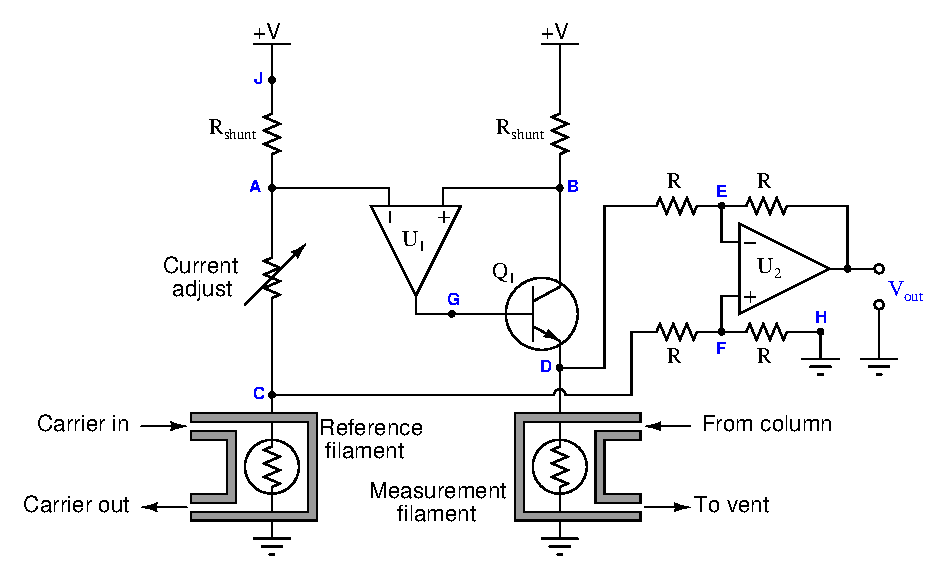
\includegraphics[width=15.5cm]{i00678x02.eps}$$

\filbreak \vskip 20pt \vbox{\hrule \hbox{\strut \vrule{} {\bf Virtuell feilsøking} \vrule} \hrule}

\noindent
{\bf Forutsi effekt av gitt feil:} presenter hver av følgende feil for studentene, én om gangen, og la dem kommentere alle effekter hver feil gir.

\begin{itemize}
\item{}
\item{}
\item{}
\end{itemize}


\vskip 10pt


\noindent
{\bf Identifisere mulige/umulige feil:} presenter symptomer og la studentene avgjøre om foreslåtte feil kan forklare alle symptomene.

\begin{itemize}
\item{} Symptom: {\it }
\item{}  -- {\bf Ja/Nei}
\item{}  -- {\bf Ja/Nei}
\item{}  -- {\bf Ja/Nei}
\end{itemize}


\vskip 10pt


\noindent
{\bf Vurdere nytten av diagnostiske tester:} presenter symptomer og foreslå følgende tester én etter én.

\begin{itemize}
\item{} Symptom: {\it $V_{out}$ er "pegged" fullt positiv}
\item{} Mål $V_{JH}$ -- {\bf Nei}
\item{} Mål $V_{CH}$ -- {\bf Ja}
\item{} Mål $V_{DH}$ -- {\bf Ja}
\item{} Mål $V_{JA}$ -- {\bf Ja}
\item{} Mål $V_{JB}$ -- {\bf Ja}
\item{} Mål $V_{EF}$ -- {\bf Ja}
\end{itemize}


\vskip 10pt


\noindent
{\bf Diagnostisere feil fra symptomer:} tenk deg at ??? feiler ??? i systemet (ikke avslør feilen). Presenter operatørens observasjon(er), la studentene foreslå tester, og gi resultater fortløpende til feilen er identifisert.

\begin{itemize}
\item{} Operatørobservasjon: {\it }
\item{}
\item{}
\end{itemize}
%INDEX% Måling, analytisk: kromatografi

%(END_NOTES)
